\documentclass[tikz,border=10pt]{standalone}
\usepackage{tikz}
\usetikzlibrary{positioning}
\usepackage{tikz-feynman}
\begin{document}

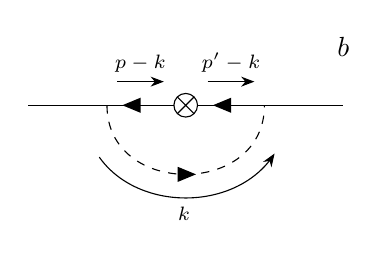
\begin{tikzpicture}
	\begin{feynman}
		%% fig a
		\vertex (a1) at (0,0);
		%% fig b
		\vertex[above right =1cm and 5cm of a1] (b1);
		\vertex[right =1cm  of b1] (b2);
		\vertex[right =2cm  of b1,crossed dot,anchor=center] (b3){};
		\vertex[right =3cm  of b1] (b4);
		\vertex[right =4cm  of b1] (b5);
		\node[above =0.5 of b5] {$b$};
		% 对各个顶点连线
		\diagram*{
		{ [edge=anti fermion]
		(b2) --[momentum={\scriptsize \(p-k\)}]  (b3)-- [momentum={\scriptsize \(p^{\prime}-k\)}] (b4),
		},
		{ [edge=plain]
				(b1) --  (b2), (b4)-- (b5),
			},
		% 介子连线
		{ [edge= charged scalar]
		%(a2) --[quarter left, momentum={\scriptsize \(k\)}](a6)--[quarter left,momentum={\scriptsize \(k+q\)}](a4), 
		(b2) -- [half right, momentum'={\scriptsize \(k\)} ](b4),
		}
		};
	\end{feynman}
\end{tikzpicture}


\end{document}
